\documentclass{beamer}
\usepackage{beamerthemeshadow}
\usepackage{graphicx}
\usepackage{color}
\usepackage[utf8]{inputenc}
\usepackage{hyperref}
\usepackage[flushleft]{threeparttable}
\usepackage[english,serbian]{babel}
\definecolor{banana}{rgb}{0.53, 0.66, 0.42}
\usecolortheme[RGB={0,100,50}]{structure}

\def\d{{\fontencoding{T1}\selectfont\dj}}
\def\D{{\fontencoding{T1}\selectfont\DJ}}


\title{Tehničko i naučno pisanje}
\subtitle{-- DALL-E 2 - OpenAI --}
\author{Ognjen Marković, Bogdan Milovanović, Matija Milovanović, Bojana Radovanović}
\institute{Matematički fakultet\\Univerzitet u Beogradu}
\date{
	\footnotesize{Beograd, 2022.}	
}

\begin{document}
\begin{frame}
	\thispagestyle{empty}
	\titlepage
\end{frame}

\addtocounter{framenumber}{-1}

\begin{frame}[fragile]\frametitle{Literatura}
	\begin{itemize}
		\item Zasnovano na seminarskom radu: DALL-E 2 - OpenAI
		(\url{https://github.com/OgnjenMarkoviic/26_TNP_2022/blob/main/DALL%20E%202%20-%20OpenAI.pdf/})
	\end{itemize}
\end{frame}

\begin{frame}
	\frametitle{Pregled} % Table of contents slide, comment this block out to remove it
	\tableofcontents[] 
\end{frame}

\section{DALL-E 2}
\subsection{Veštačka inteligencija i tehnologija}
\begin{frame}[fragile]\frametitle{Veštačka inteligencija i tehnologija}
	\begin{itemize}	
		\item Prvobitna definicija AI-a
		\item Princip rada (algoritmika, pretraga, deduktivno i induktivno zaključivanje, itd.)
		\item Primena veštačke inteligencije
		\item NLP - interakcija izmteđu računara i ljudskog jezika
		\item GPT
		\item DALL-E 2
        \begin{table}[h!]
        \begin{center}
        \vspace{0.5cm}
        \begin{tabular}{|c|c|c|c|c|} \hline
        2018&2019&2020&2021&2022\\ \hline
        GPT&GPT-2&GPT-3 &DALL-E&DALL-E 2\\ \hline
        \end{tabular}
        \label{tab:tabela1}
        \caption{Hronološki razvitak DALL-E 2.}
        \end{center}
        \end{table}
	\end{itemize}
\end{frame}

\subsection{Mogućnosti}

\begin{frame}[fragile]\frametitle{Mogućnosti I}
	DALL-E 2 može da:
    \begin{itemize}
        \item generiše slike u više stilova, uključujući fotorealistične slike i emotikone
        \item da manipuliše i preuređuje objekte na svojim slikama
        \item ispravno postavi elemente dizajna u nove kompozicije bez eksplicitnih instrukcija
    \end{itemize}
    \newpage
\end{frame}

\begin{frame}[fragile]\frametitle{Mogućnosti II}
	Neke zanimljive slike generisane pomoću DALL-E 2 softvera:
	\begin{figure}%
    \centering
    \subfloat{{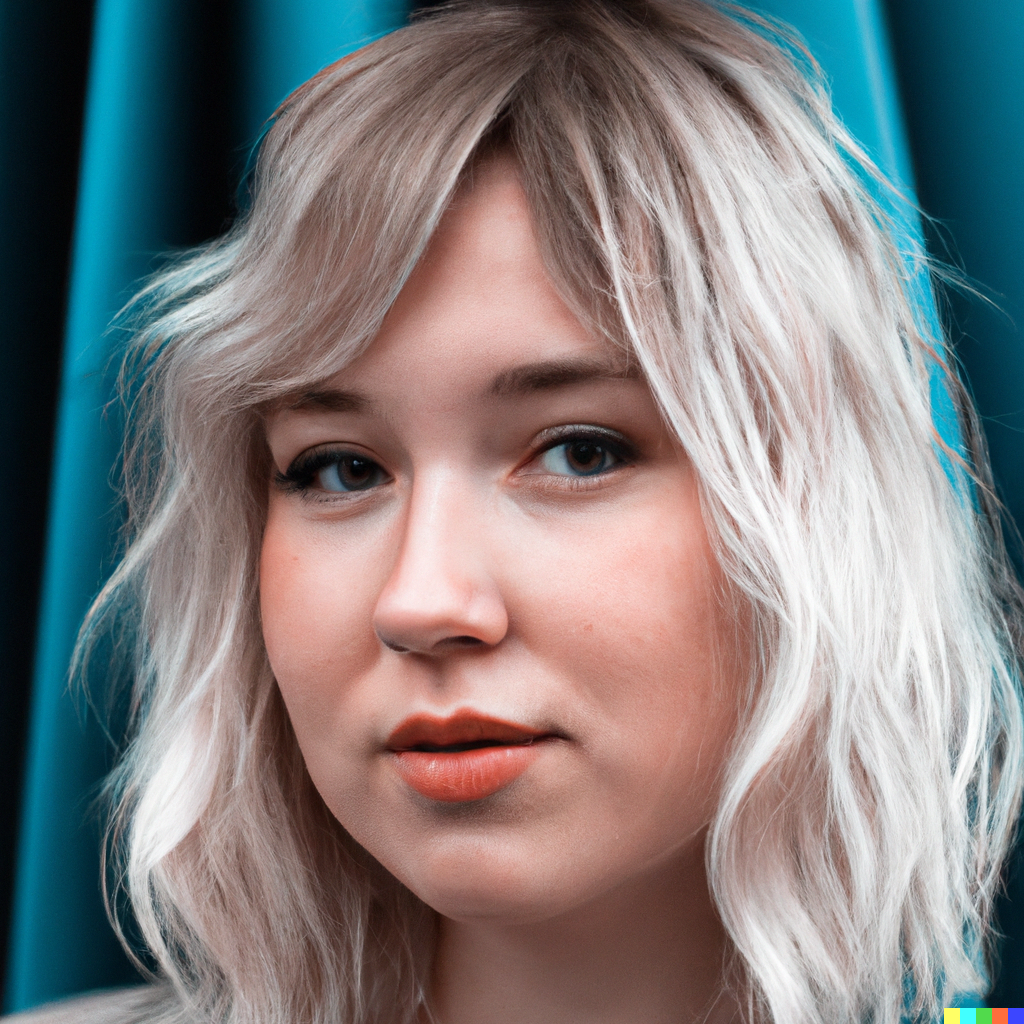
\includegraphics[scale=0.08]{zena.jpg} }}%
    \qquad
    \subfloat{{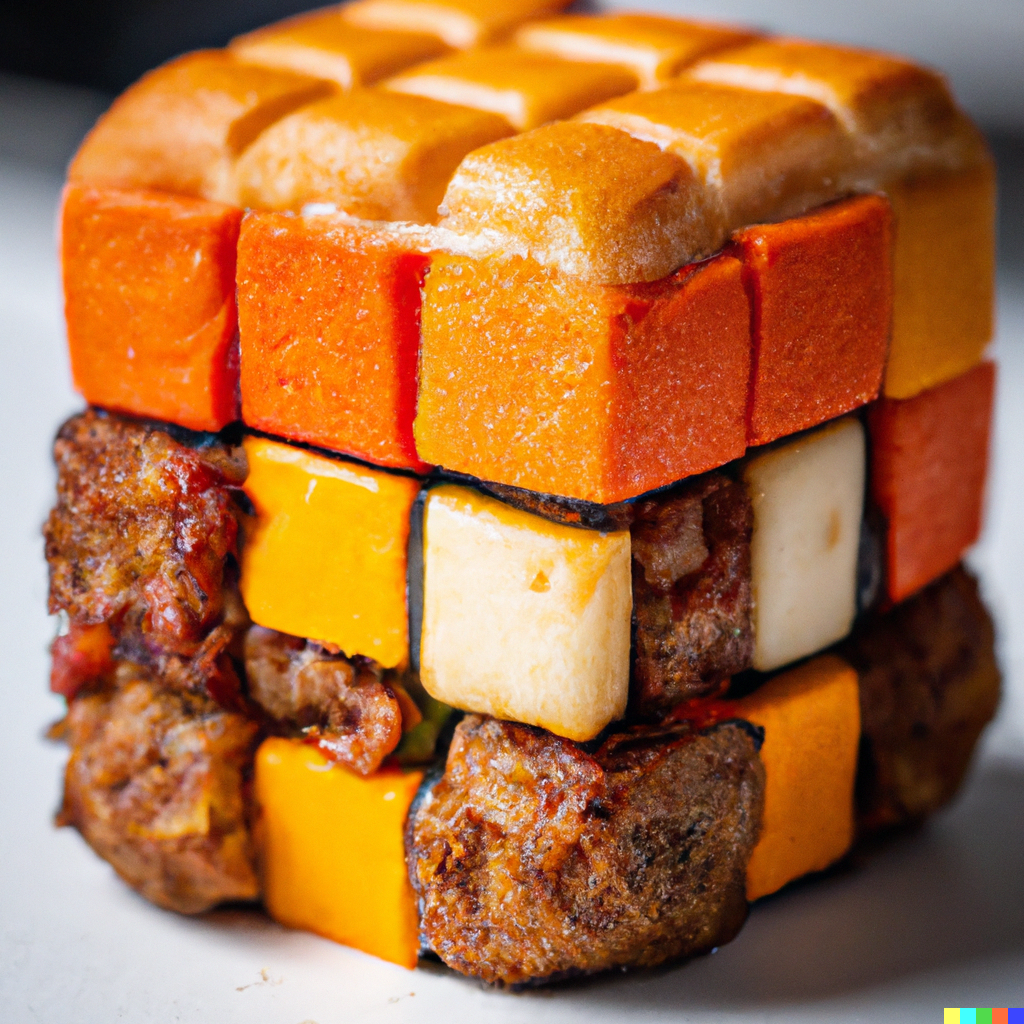
\includegraphics[scale=0.08]{hamburger.jpg} }}%
    \qquad
    \subfloat{{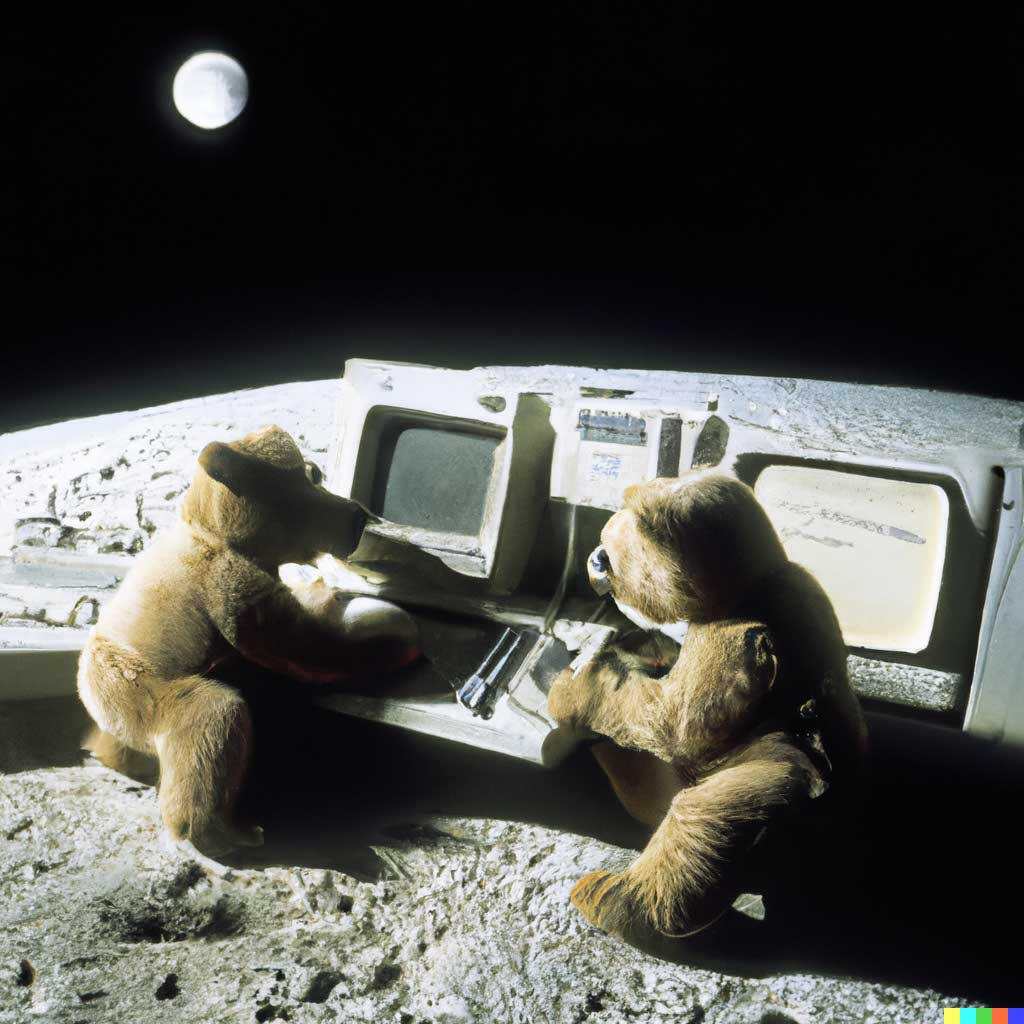
\includegraphics[scale=0.08]{medvedi.jpg} }}%
 
    \label{fig:example}
    \end{figure}
\end{frame}

\subsection{Etički problemi i tehnička ograničenja}

\begin{frame}[fragile]\frametitle{Etički problemi i tehnička ograničenja}
	\begin{itemize}	
		\item Zloupotreba generisanih slika
		\item Filtriranje teksta
		\item Duboki fejkovi
		\item Izuzetna konkurencija umetničkom stvaralaštvu
		\item Leksički problemi - besmislene reči
		\item Semantički problemi - konj koji jaše astronauta - astronaut koji jaše konja
		\item Količina unetih podataka
	\end{itemize}
\end{frame}

\section{Zaključak}

\begin{frame}[fragile]\frametitle{Zaključak}
	\item DALL-E 2 je softver koji predstavlja minijaturnu primenu veštačke inteligencije i pokazuje koliko ona može biti fascinantna i zastrašujuća samo gledajući obične slike. Veštačka inteligencija je oblast koja je u velikom usponu i naš zadatak je da je iskoristimo u humane svrhe i što manje zloupotrebimo.
\end{frame}

\section{Literatura}

\begin{frame}[fragile]\frametitle{Literatura}
	\begin{itemize}
		\item Allyn, Bobby. Surreal or too real? Breathtaking AI tool DALL-E takes
its images to a bigger stage. NPR. Retrieved 20 July 2022.
		\item OpenAI DALL·E 2 Preview - Risks and Limitations, 19 June 2022
		\item Macaulay, Thomas Say hello to OpenAI’s DALL-E, a GPT-3-powered
bot that creates weird images from text. TheNextWeb, 28 January 2021.
        \item Sahar Mor, Stripe "How DALL-E 2 could solve major computer vision
challenges".
        \item Walsh, Bryan "A new AI model draws images from text"
	\end{itemize}
\end{frame}



\end{document}